\chapter{Searching for an \textit{(un)stable equilibrium}:
Experiments in Training Generative Neural Networks Without Data}
\label{ch:unstable_eq}

\section{Introduction}

This chapter details the first successful attempt in my PhD research in finding a way of training a generative neural network in a data divergent (or data agnostic) way. 
This work is one of the first recorded endeavours of training a generative neural network without training data, alongside Joel Simon’s excellent work Dimensions of dialogue [\citeyear{simon2019dimensions}]. 
These works were done concurrently and independently of each other, and were disseminated at around the same time \footnote{Joel Simons Blog does not contain a date, so I cannot determine an exact chronology here}. 

This work was published as a short paper at the NerIPS 2019 Workshop on Machine Learning for Creativity and Design, in Vancouver, Canada \citep{broad2019searching}. 
Chapter \ref{ch:impact} details the reception of the series of artworks \textit{(un)stable equilibrium} that resulted from these experiments. 

\begin{figure}[!htbp]
    \centering
    \subfloat[]{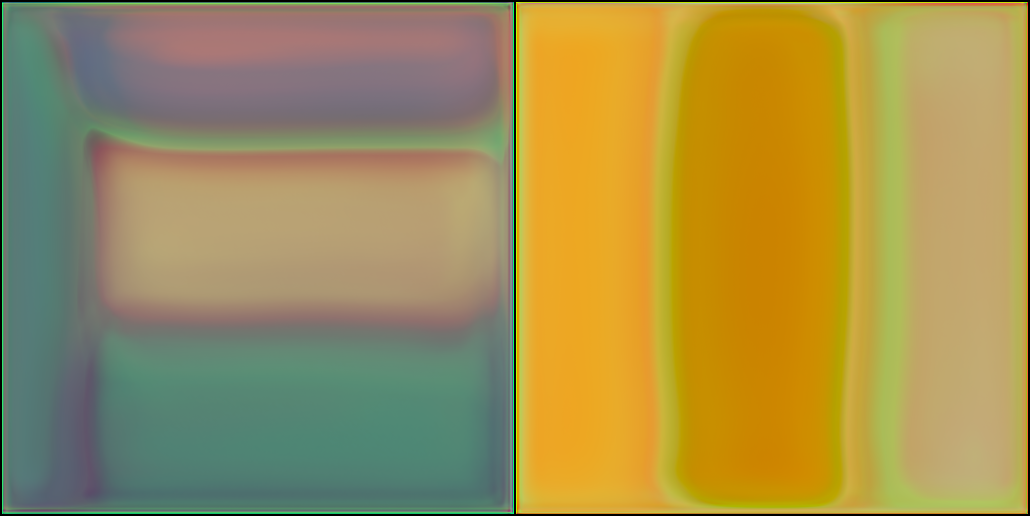
\includegraphics[width=0.45\textwidth]{figures/c4_unstable/original_experiments/1_1.png}}
    \hfill
    \subfloat[]{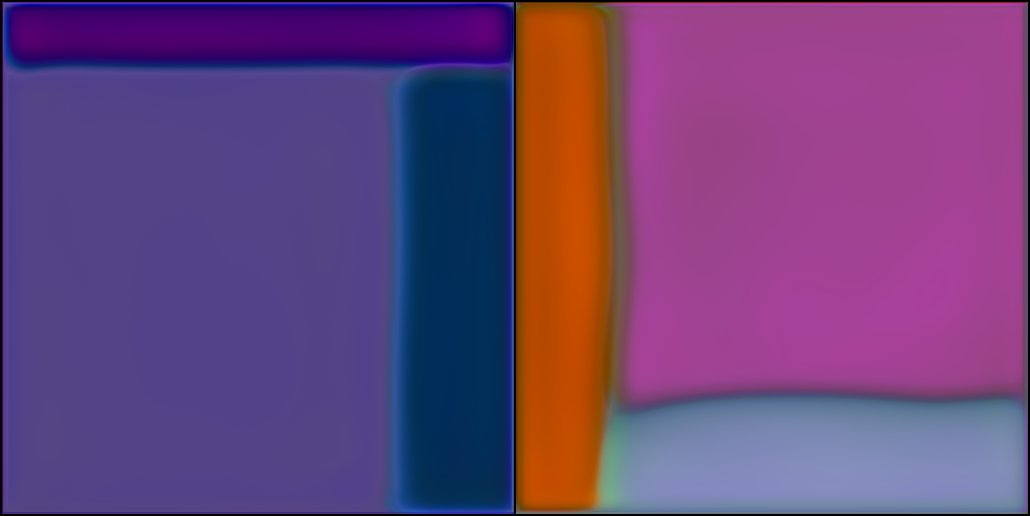
\includegraphics[width=0.45\textwidth]{figures/c4_unstable/original_experiments/1_2.png}}
    \hfill
    \subfloat[]{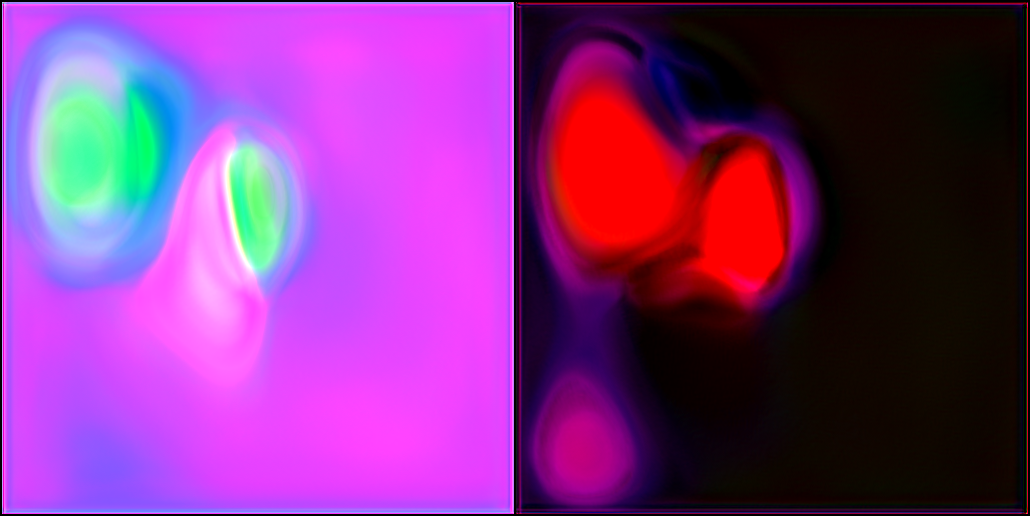
\includegraphics[width=0.45\textwidth]{figures/c4_unstable/original_experiments/1_3.png}}
    \hfill
    \subfloat[]{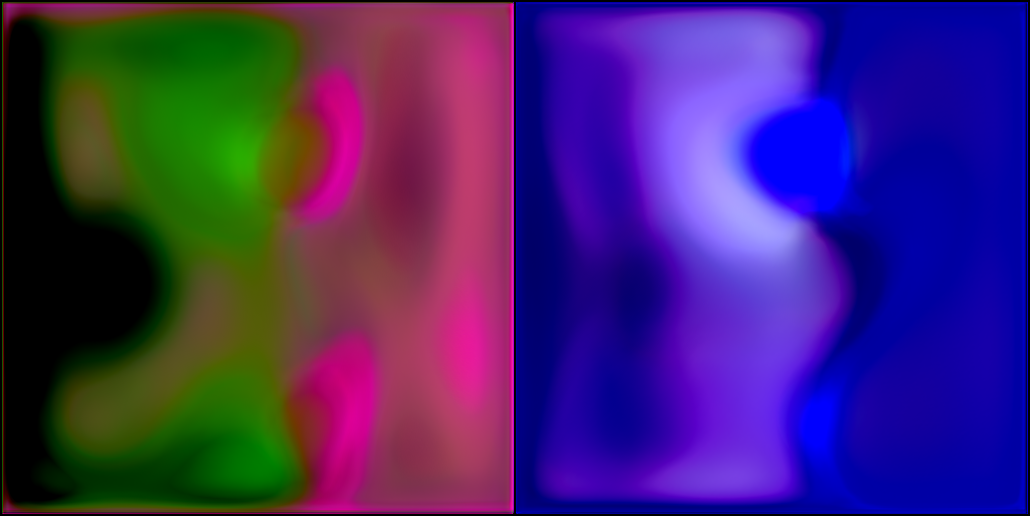
\includegraphics[width=0.45\textwidth]{figures/c4_unstable/original_experiments/1_4.png}}
    \hfill
    \subfloat[]{
\includegraphics[width=0.45\textwidth]{figures/c4_unstable/original_experiments/1_5.png}}
    \hfill
    \subfloat[]{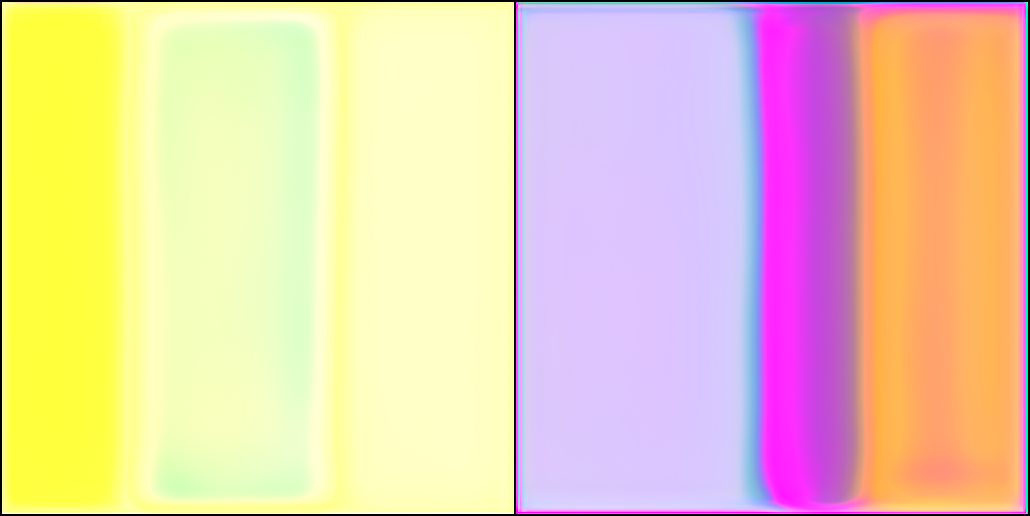
\includegraphics[width=0.45\textwidth]{figures/c4_unstable/original_experiments/1_6.png}}
    \caption[]{}
    \label{fig:c3:original-experiments}
  \end{figure}



\section{Motivation}

This work came out of a deep frustration early on in my PhD journey, where I was trying to find ways of training generative models without modelling data.
It took me far longer than it should have to come to the realisation that this is an oxymoron. 
That a generative model is a model of a data distribution, and nothing more. 
Any attempt to move past this notion needed a completely different approach, and the first approach I developed which was fruitful is what is presented in this chapter. 

This work came out of a simple proposition: if it was possible to find a way of training a generative neural network without any training data, then by default, any outcome must be novel and could not resemble an existing training data distribution. 
There was little mathematical grounding to this approach. 
Through dogged trial and error, some playful reconfiguring of the most common (at the time) way of training generative models, GANs, I was able to find a way to train generative networks without data, in ways that produced at the very least, aesthetically interesting outcomes. 

This chapter tells the story of that process. 
Through the early experiments with configurations of models and loss functions that led to unremarkable results, through to the final configuration of models and training runs that resulted in the artworks \textit{(un)stable equilibrium}.
This chapter is named as such, because the journey I went on in producing those works was one of searching -- through intuition and aesthetic exploration -- for an (un)stable equilibrium. 
A balancing act of finding a system just chaotic enough to produce enough randomness in the resulting training run that enough unpredictable dynamics would lead to configuration of the weight parameters of the model such that unpredictable (and aesthetically compelling) results would come from the generator networks. 
But not enough for the loss functions to explode during training. 
The visual results of training were monitored, both visually by me as I inspected the generated output as each training increment progressed, along with a close monitoring of the fluctuations of the various loss functions throughout training. 
Over the course of a couple of intensive weeks of working in this unorthodox way, the configuration that produced these results was discovered. 
The following sections in this chapter tell a narrative of that process and my reflections on it. 

\section{Initial experiment}

\begin{figure}[!htbp]
    \centering
    \subfloat[]{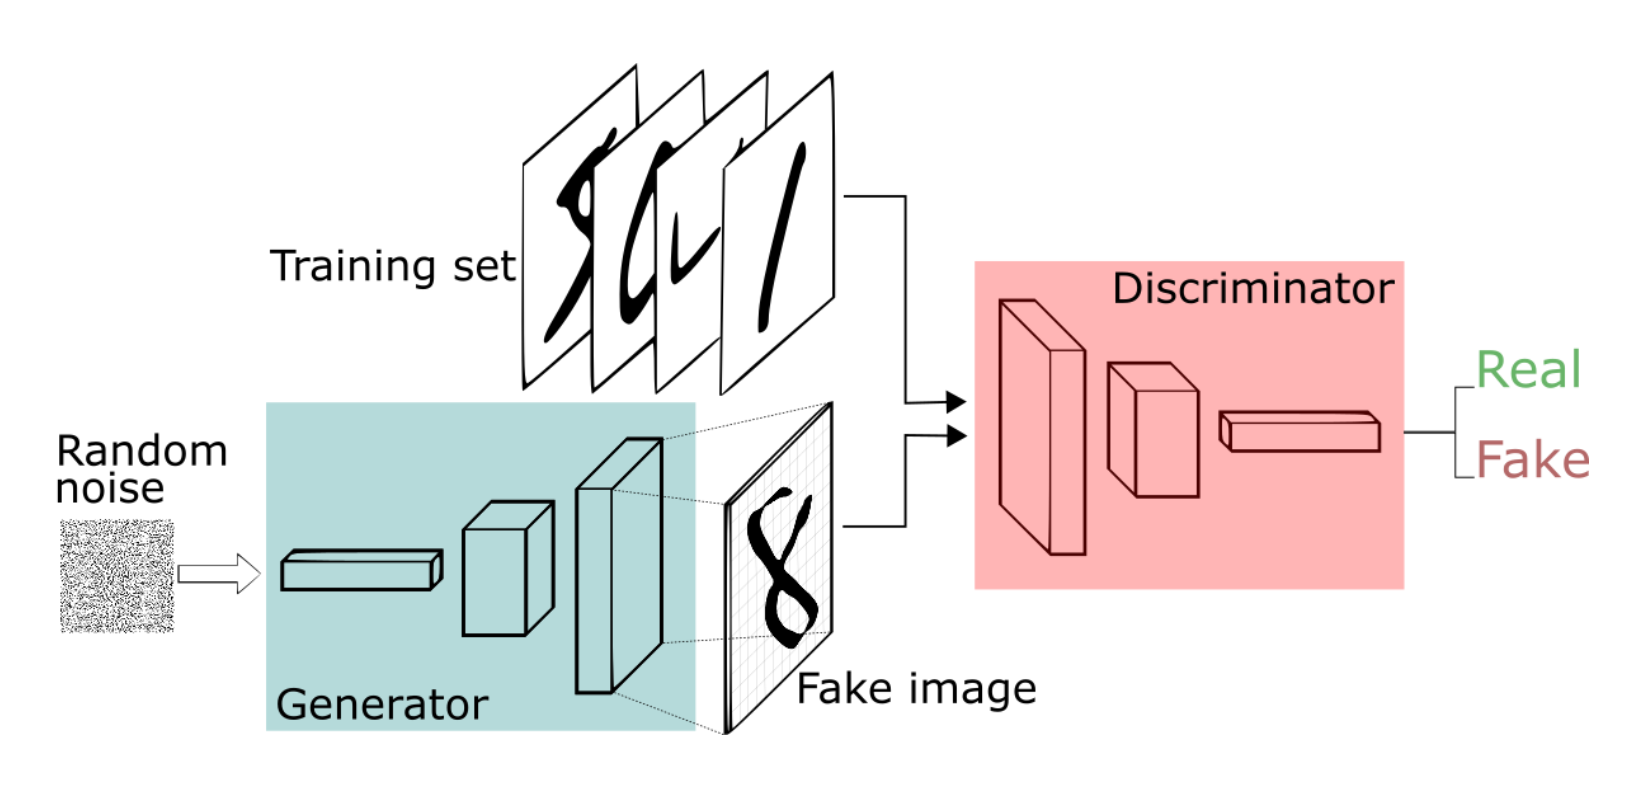
\includegraphics[width=0.75\textwidth]{figures/c4_unstable/diagrams/gan.png}}
    \hfill
    \subfloat[]{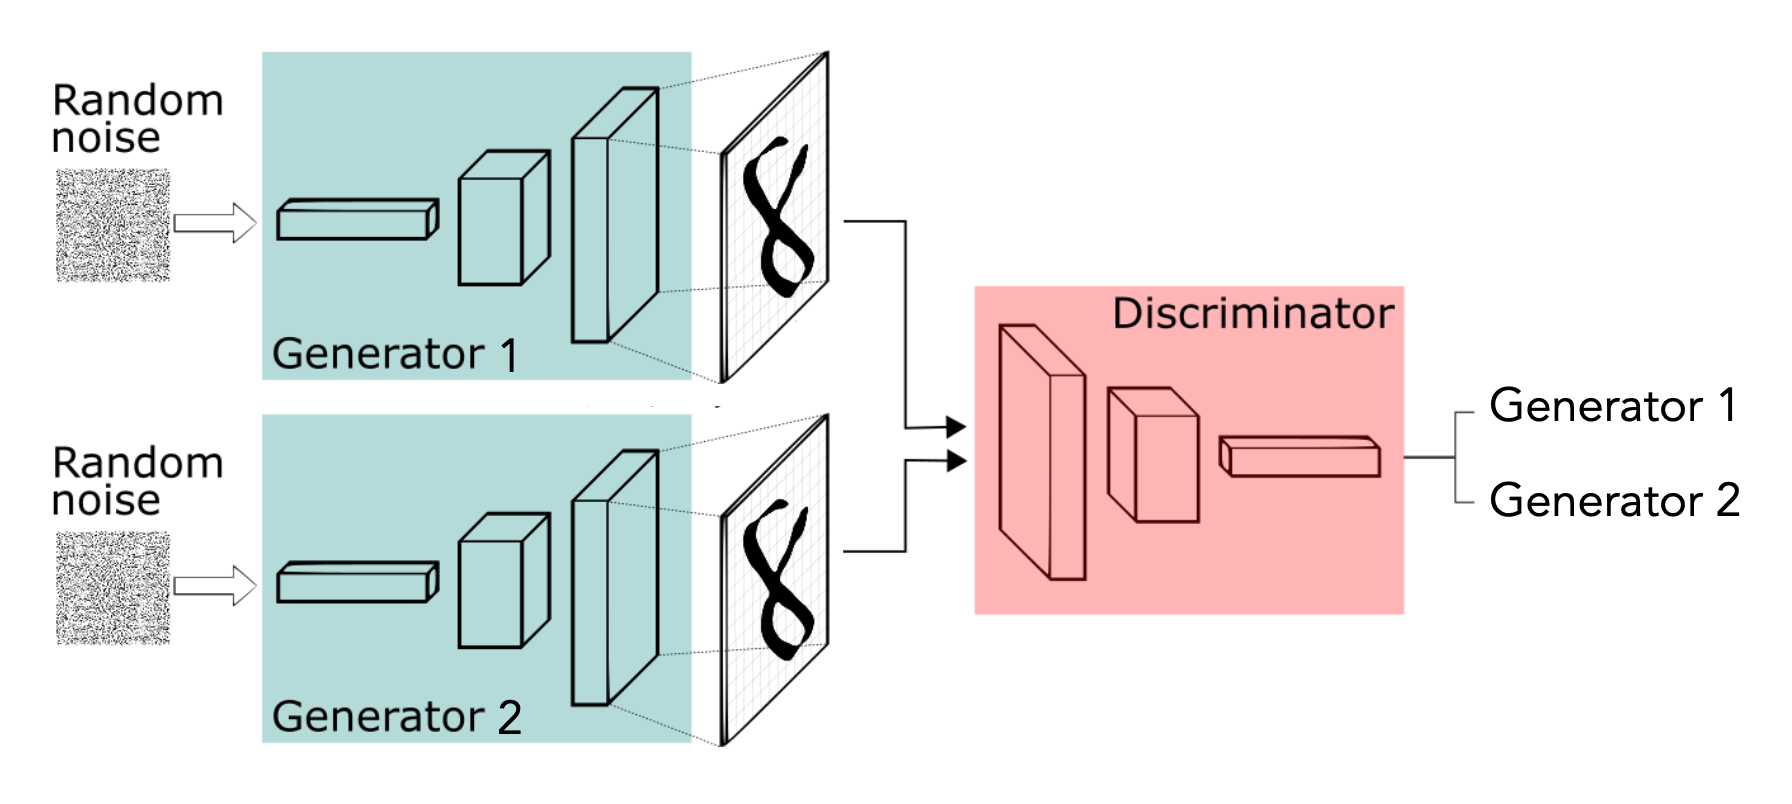
\includegraphics[width=0.75 \textwidth]{figures/c4_unstable/diagrams/two-generator.png}}
    \caption[]{}
    \label{fig:c3:gan-diagrams}
  \end{figure}

\label{c4:sec:og-loss}
\begin{figure}[!htbp]
    \centering
    \subfloat[]{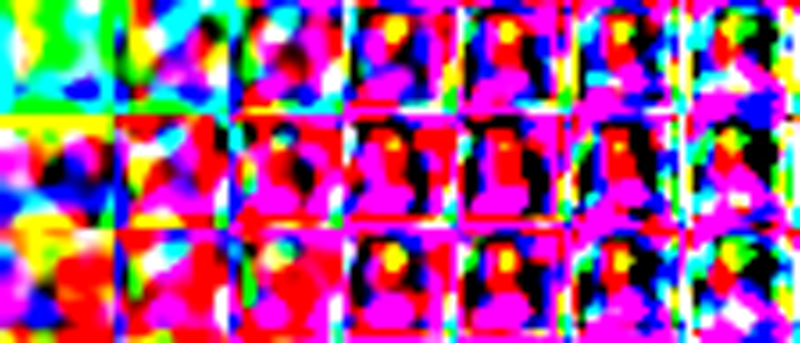
\includegraphics[width=0.45\textwidth]{figures/c4_unstable/train_samples/no_col_var/scaled_step_2_g1.png}}
    \hfill
    \subfloat[]{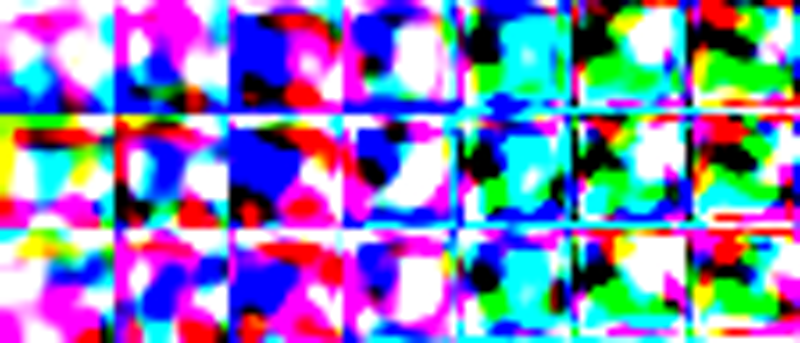
\includegraphics[width=0.45\textwidth]{figures/c4_unstable/train_samples/no_col_var/scaled_step_2_g2.png}}
    \hfill
    \subfloat[]{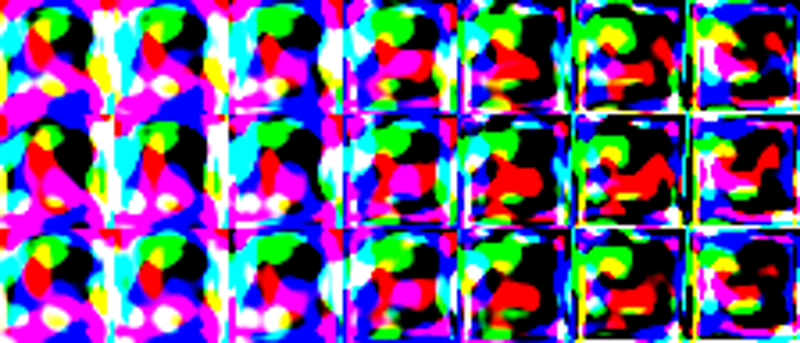
\includegraphics[width=0.45\textwidth]{figures/c4_unstable/train_samples/no_col_var/scaled_step_3_g1.png}}
    \hfill
    \subfloat[]{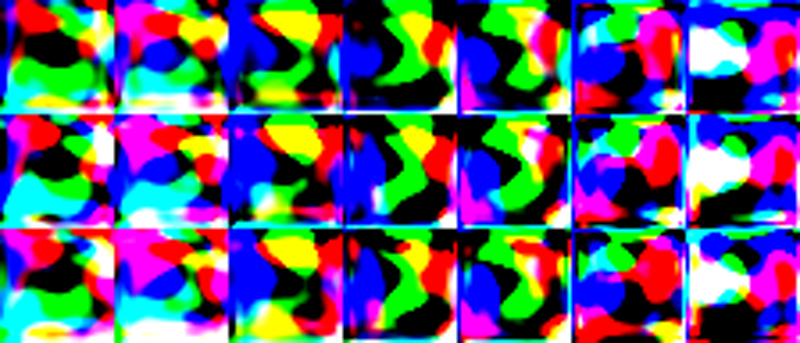
\includegraphics[width=0.45\textwidth]{figures/c4_unstable/train_samples/no_col_var/scaled_step_3_g2.png}}
    \hfill
    \subfloat[]{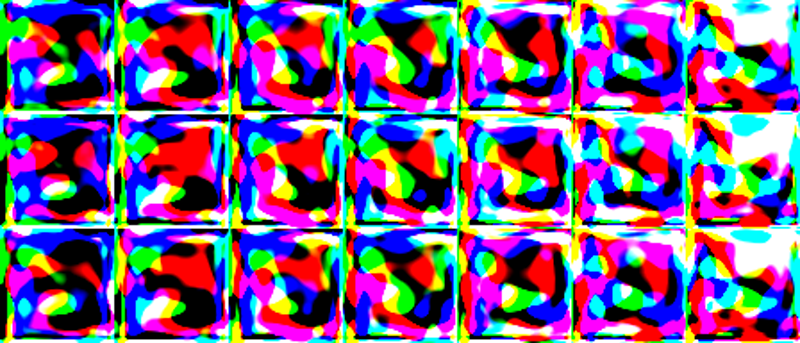
\includegraphics[width=0.45\textwidth]{figures/c4_unstable/train_samples/no_col_var/scaled_step_4_g1.png}}
    \hfill
    \subfloat[]{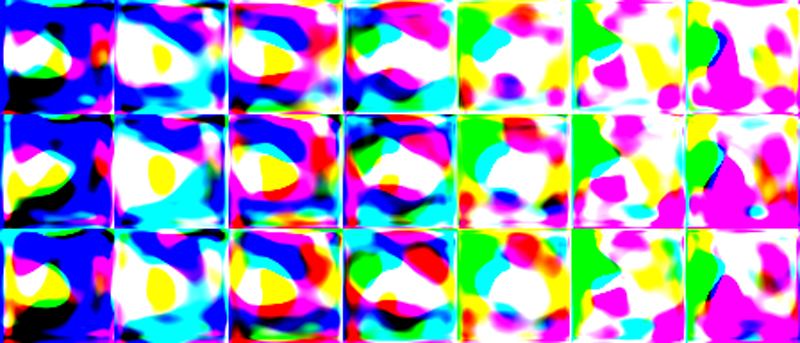
\includegraphics[width=0.45\textwidth]{figures/c4_unstable/train_samples/no_col_var/scaled_step_4_g2.png}}
    \hfill
    \subfloat[]{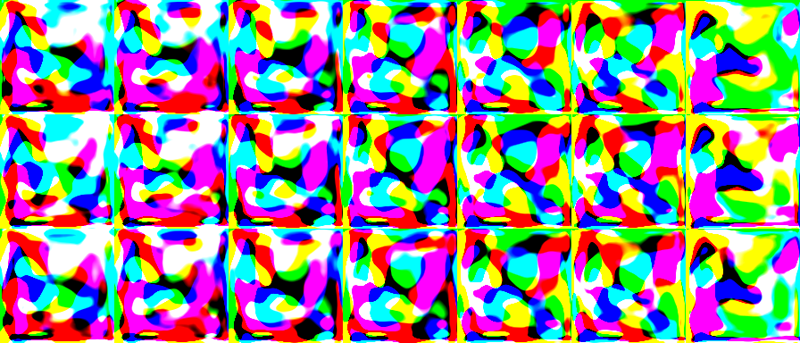
\includegraphics[width=0.45\textwidth]{figures/c4_unstable/train_samples/no_col_var/scaled_step_5_g1.png}}
    \hfill
    \subfloat[]{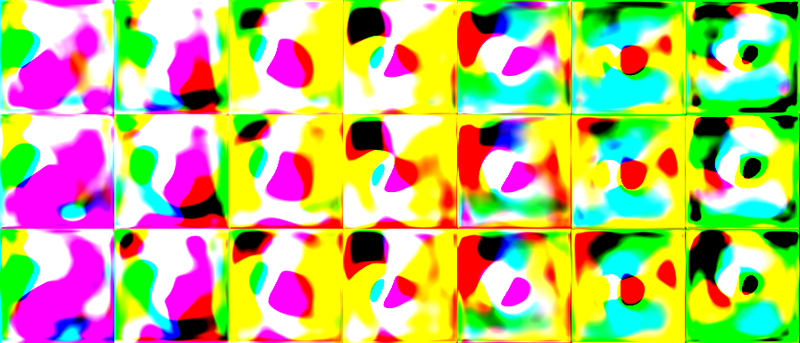
\includegraphics[width=0.45\textwidth]{figures/c4_unstable/train_samples/no_col_var/scaled_step_5_g2.png}}
    \hfill
    \subfloat[]{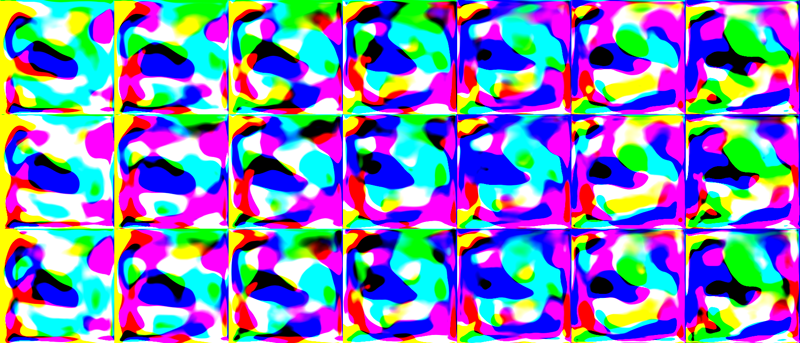
\includegraphics[width=0.45\textwidth]{figures/c4_unstable/train_samples/no_col_var/scaled_step_6_g1.png}}
    \hfill
    \subfloat[]{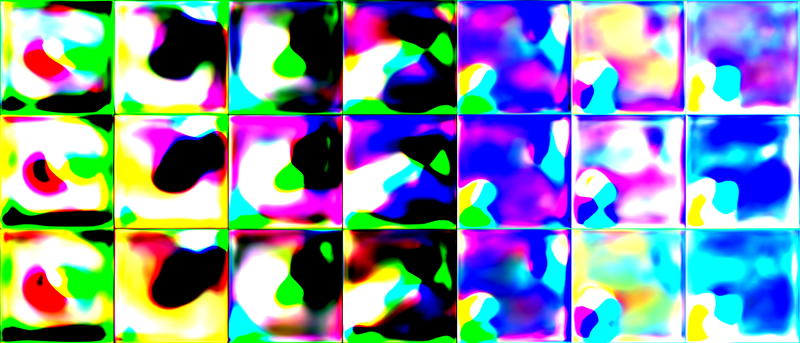
\includegraphics[width=0.45\textwidth]{figures/c4_unstable/train_samples/no_col_var/scaled_step_6_g2.png}}
    \hfill
    \caption[]{}
    \label{fig:c3:samples-no-col-var}
  \end{figure}

  \begin{figure}[!htbp]
    \centering
    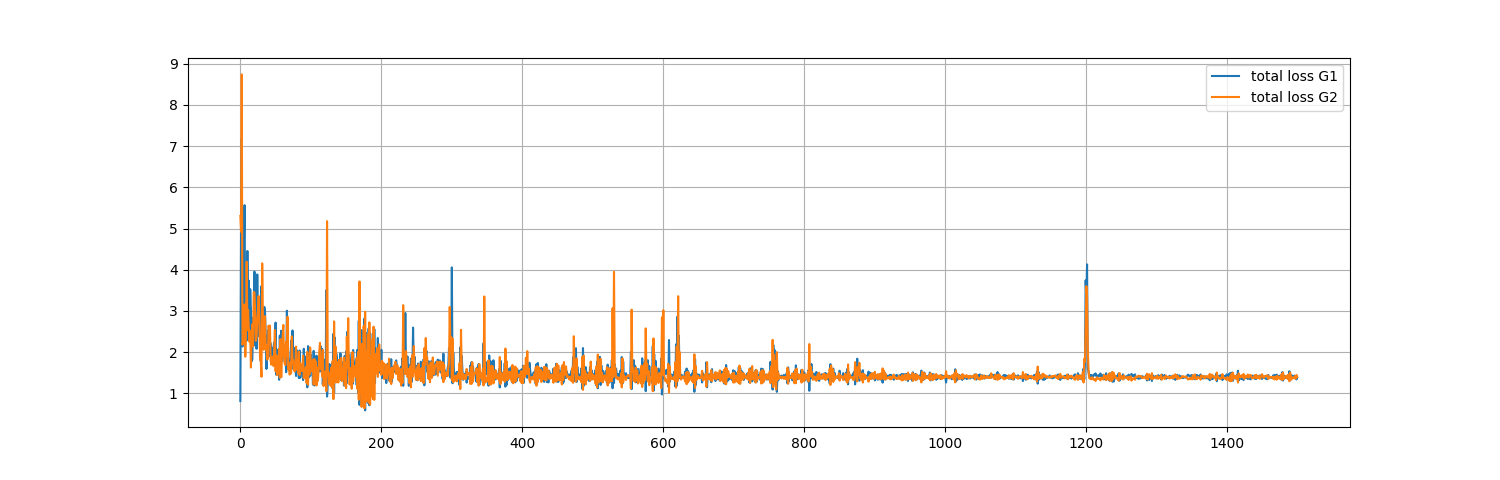
\includegraphics[width=1\textwidth]{figures/c4_unstable/train_losses/no_col_var/total_loss_no_var.png}
    \label{fig:c3:no-var-losses}
  \end{figure}

\section{Colour variance loss}

\begin{figure}[!htbp]
    \centering
    \subfloat[]{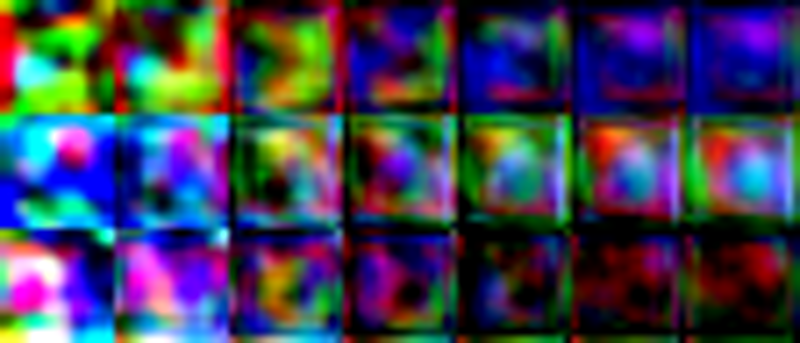
\includegraphics[width=0.45\textwidth]{figures/c4_unstable/train_samples/col_var/scaled_step_2_g1.png}}
    \hfill
    \subfloat[]{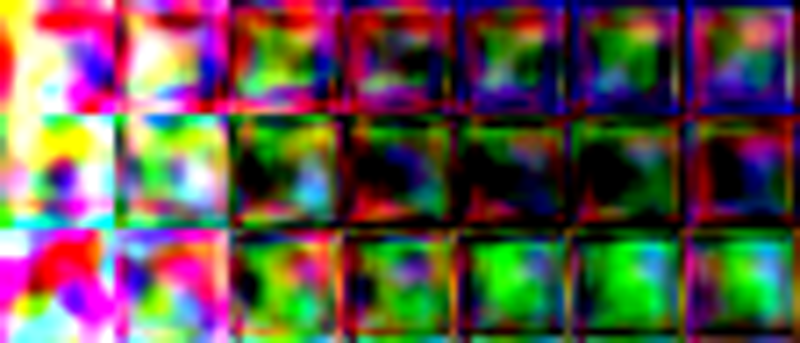
\includegraphics[width=0.45\textwidth]{figures/c4_unstable/train_samples/col_var/scaled_step_2_g2.png}}
    \hfill
    \subfloat[]{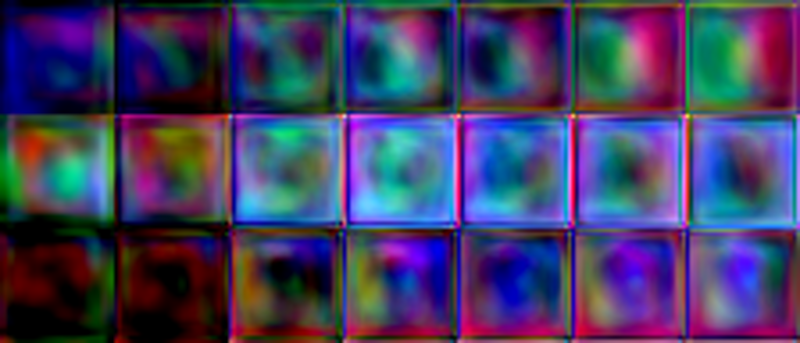
\includegraphics[width=0.45\textwidth]{figures/c4_unstable/train_samples/col_var/scaled_step_3_g1.png}}
    \hfill
    \subfloat[]{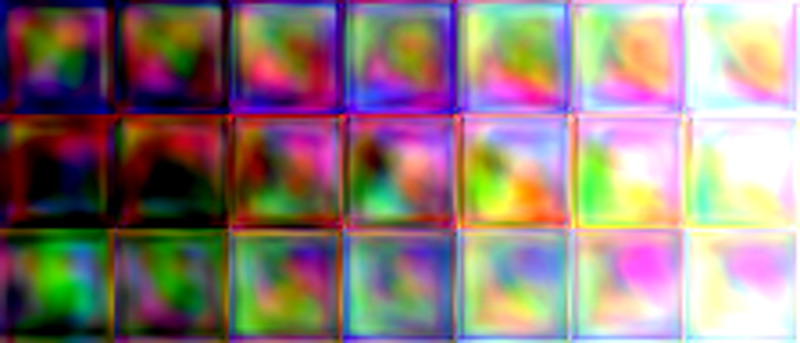
\includegraphics[width=0.45\textwidth]{figures/c4_unstable/train_samples/col_var/scaled_step_3_g2.png}}
    \hfill
    \subfloat[]{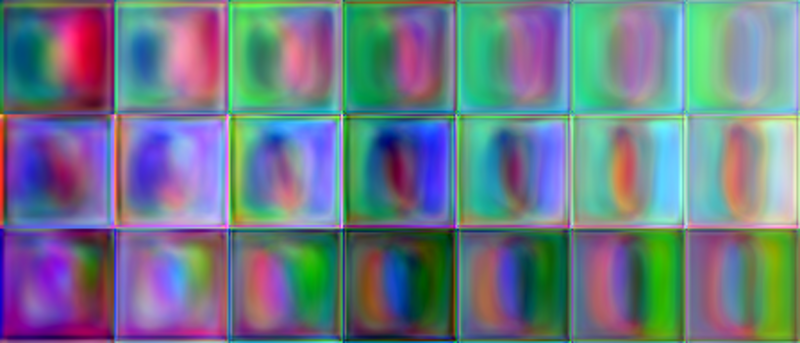
\includegraphics[width=0.45\textwidth]{figures/c4_unstable/train_samples/col_var/scaled_step_4_g1.png}}
    \hfill
    \subfloat[]{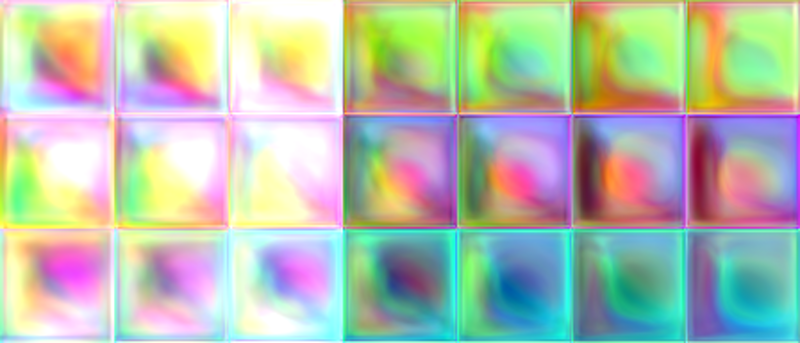
\includegraphics[width=0.45\textwidth]{figures/c4_unstable/train_samples/col_var/scaled_step_4_g2.png}}
    \hfill
    \subfloat[]{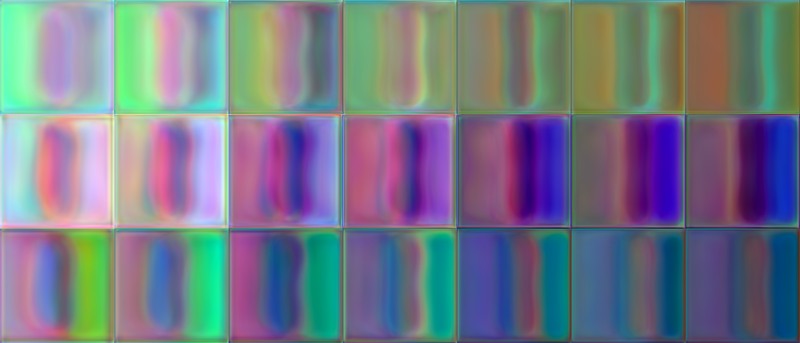
\includegraphics[width=0.45\textwidth]{figures/c4_unstable/train_samples/col_var/scaled_step_5_g1.png}}
    \hfill
    \subfloat[]{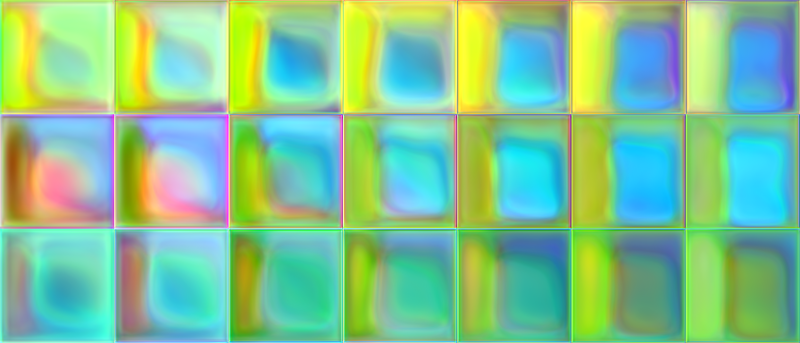
\includegraphics[width=0.45\textwidth]{figures/c4_unstable/train_samples/col_var/scaled_step_5_g2.png}}
    \hfill
    \subfloat[]{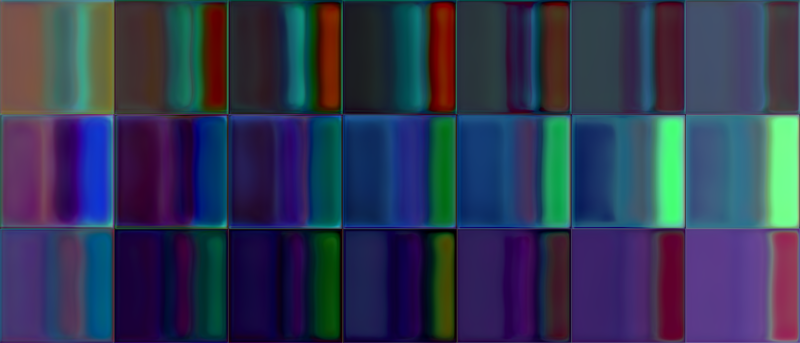
\includegraphics[width=0.45\textwidth]{figures/c4_unstable/train_samples/col_var/scaled_step_6_g1.png}}
    \hfill
    \subfloat[]{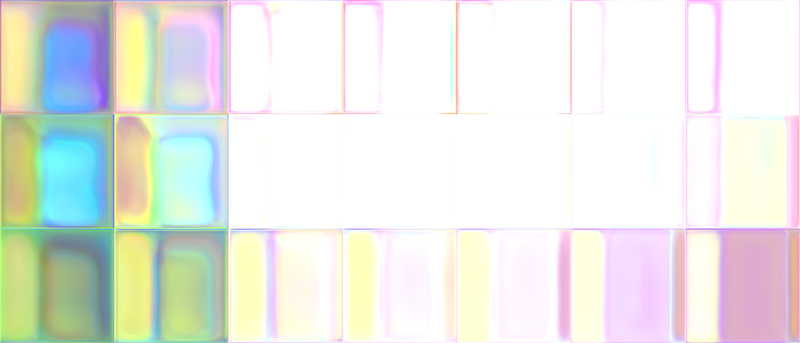
\includegraphics[width=0.45\textwidth]{figures/c4_unstable/train_samples/col_var/scaled_step_6_g2.png}}
    \hfill
    \caption[]{}
    \label{fig:c3:samples-col-var}
  \end{figure}

  \begin{figure}[!htbp]
    \centering
    \subfloat[]{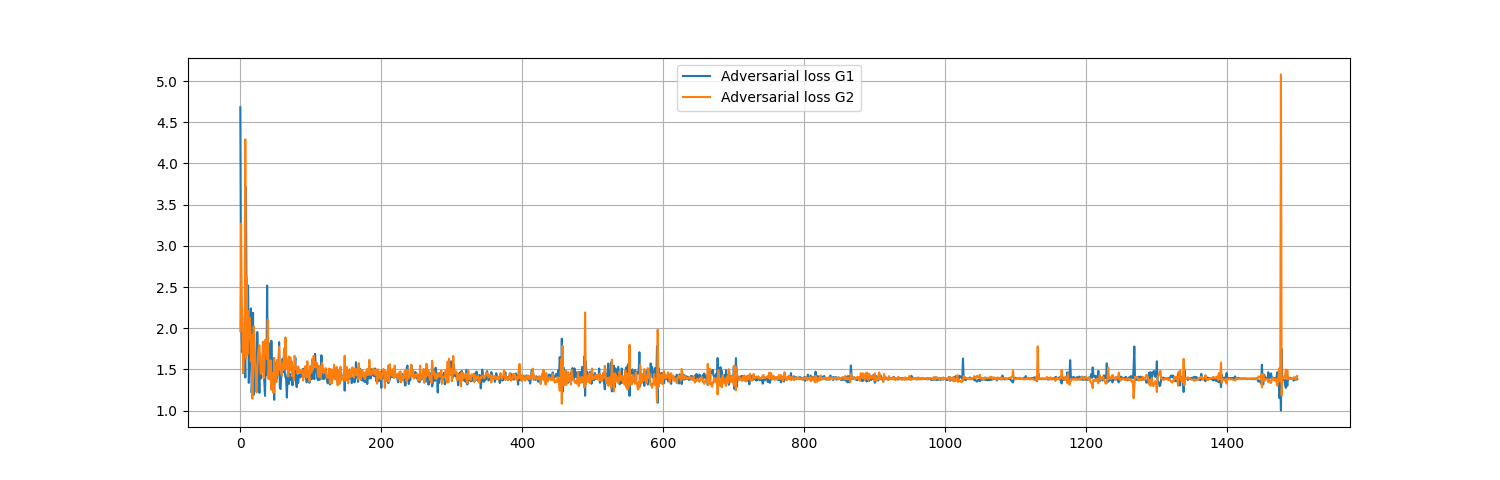
\includegraphics[width=1\textwidth]{figures/c4_unstable/train_losses/col_var/adversarial_loss.png}}
    \hfill
    \subfloat[]{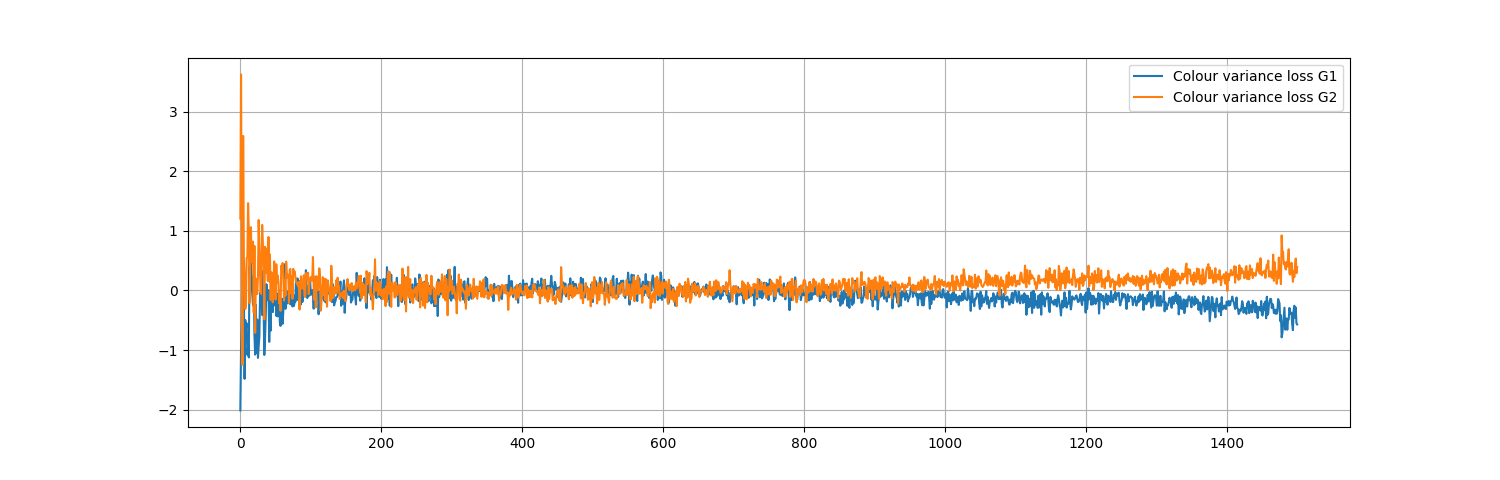
\includegraphics[width=1\textwidth]{figures/c4_unstable/train_losses/col_var/col_var_loss.png}}
    \hfill
    \subfloat[]{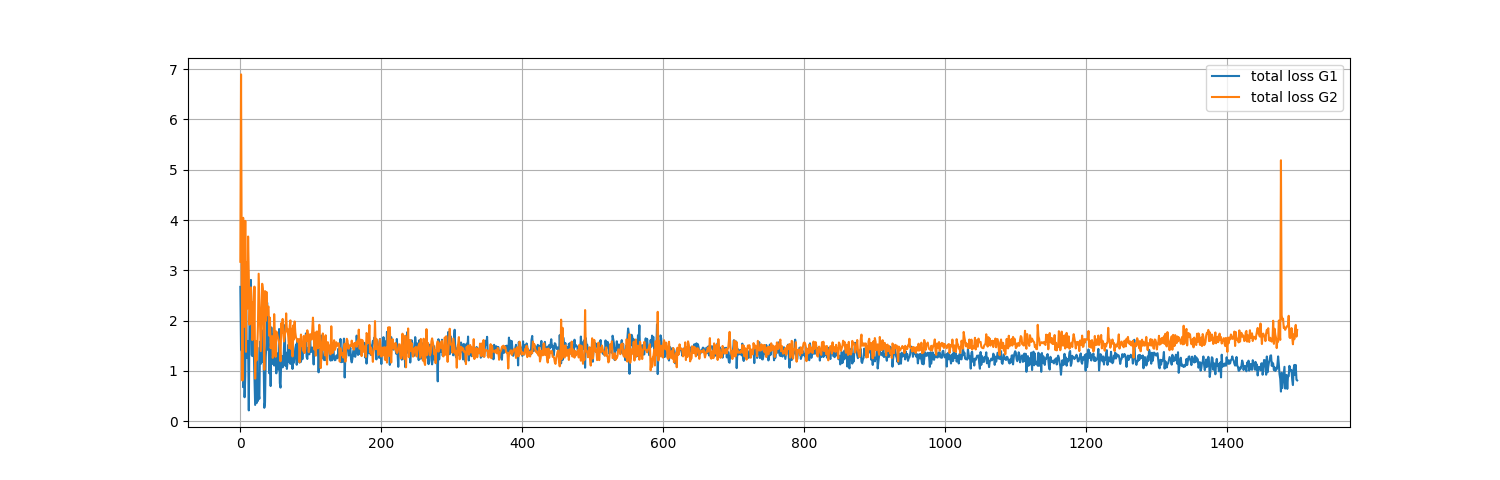
\includegraphics[width=1\textwidth]{figures/c4_unstable/train_losses/col_var/total_loss.png}}
    \caption[]{}
    \label{fig:c3:col-var-losses}
  \end{figure}

  
\section{Distance functions}

\section{Cosine distance}

\begin{figure}[!htbp]
    \centering
    \subfloat[]{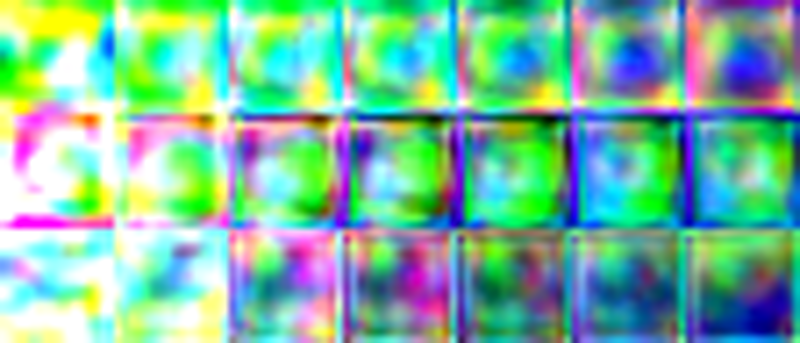
\includegraphics[width=0.45\textwidth]{figures/c4_unstable/train_samples/cos_cos/scaled_step_2_g1.png}}
    \hfill
    \subfloat[]{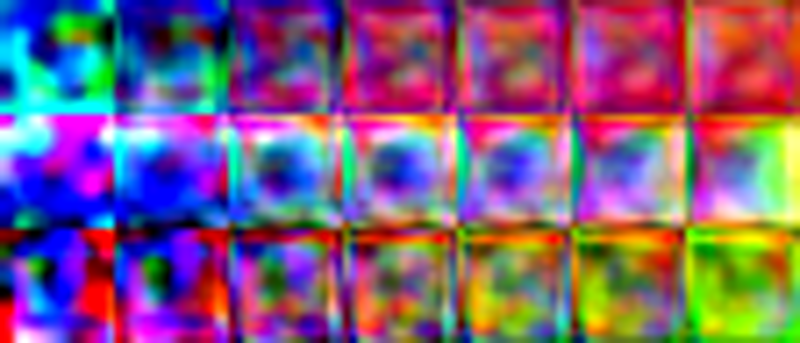
\includegraphics[width=0.45\textwidth]{figures/c4_unstable/train_samples/cos_cos/scaled_step_2_g2.png}}
    \hfill
    \subfloat[]{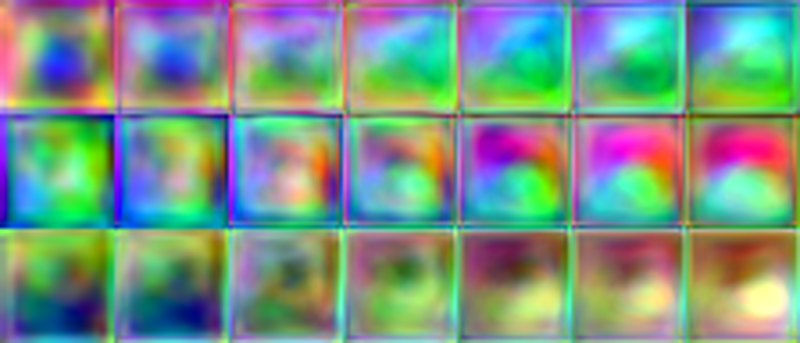
\includegraphics[width=0.45\textwidth]{figures/c4_unstable/train_samples/cos_cos/scaled_step_3_g1.png}}
    \hfill
    \subfloat[]{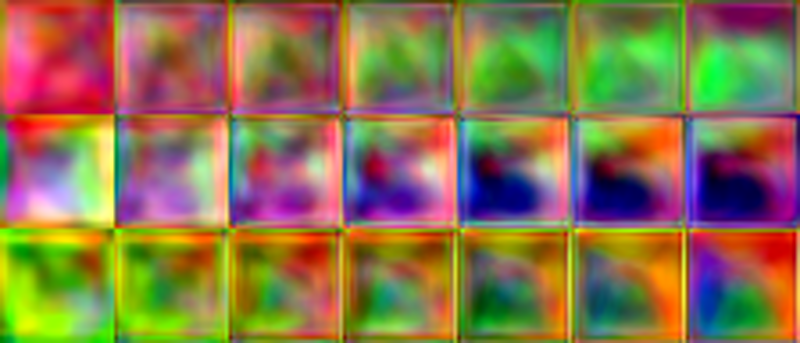
\includegraphics[width=0.45\textwidth]{figures/c4_unstable/train_samples/cos_cos/scaled_step_3_g2.png}}
    \hfill
    \subfloat[]{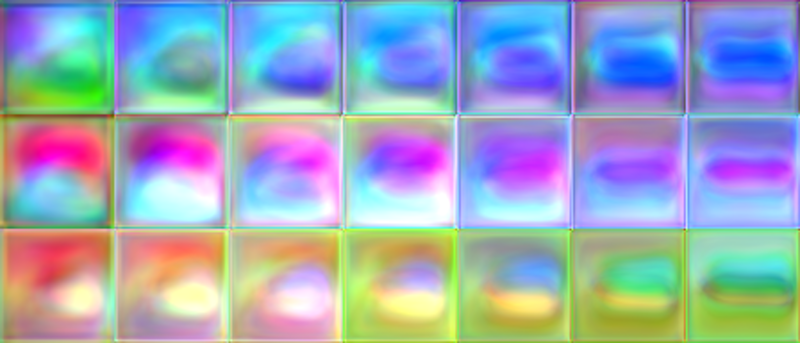
\includegraphics[width=0.45\textwidth]{figures/c4_unstable/train_samples/cos_cos/scaled_step_4_g1.png}}
    \hfill
    \subfloat[]{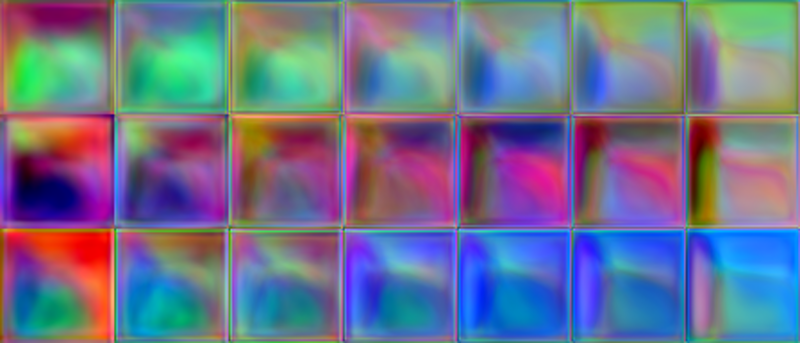
\includegraphics[width=0.45\textwidth]{figures/c4_unstable/train_samples/cos_cos/scaled_step_4_g2.png}}
    \hfill
    \subfloat[]{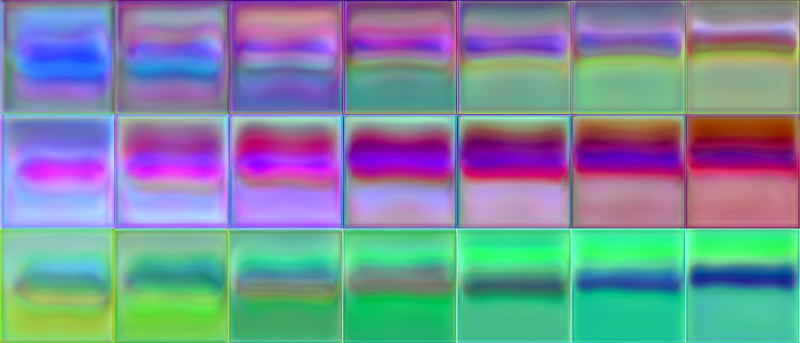
\includegraphics[width=0.45\textwidth]{figures/c4_unstable/train_samples/cos_cos/scaled_step_5_g1.png}}
    \hfill
    \subfloat[]{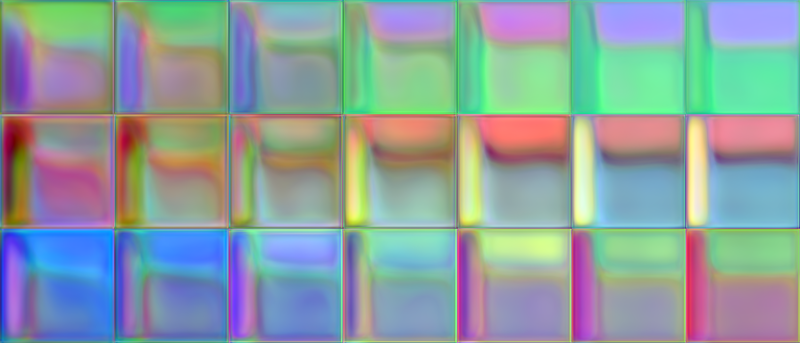
\includegraphics[width=0.45\textwidth]{figures/c4_unstable/train_samples/cos_cos/scaled_step_5_g2.png}}
    \hfill
    \subfloat[]{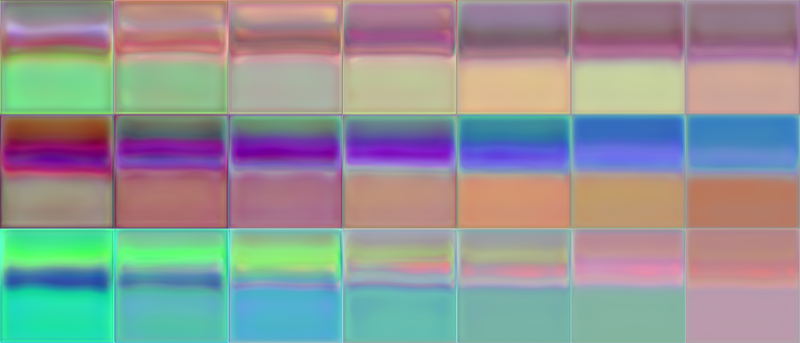
\includegraphics[width=0.45\textwidth]{figures/c4_unstable/train_samples/cos_cos/scaled_step_6_g1.png}}
    \hfill
    \subfloat[]{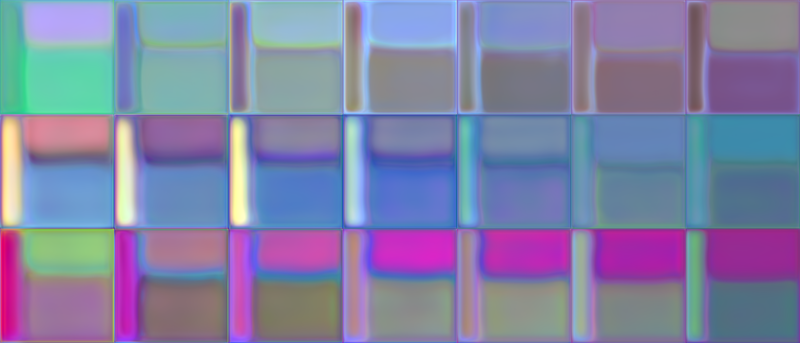
\includegraphics[width=0.45\textwidth]{figures/c4_unstable/train_samples/cos_cos/scaled_step_6_g2.png}}
    \hfill
    \caption[]{}
    \label{fig:c3:samples-cos-cos}
  \end{figure}

  \begin{figure}[!htbp]
    \centering
    \subfloat[]{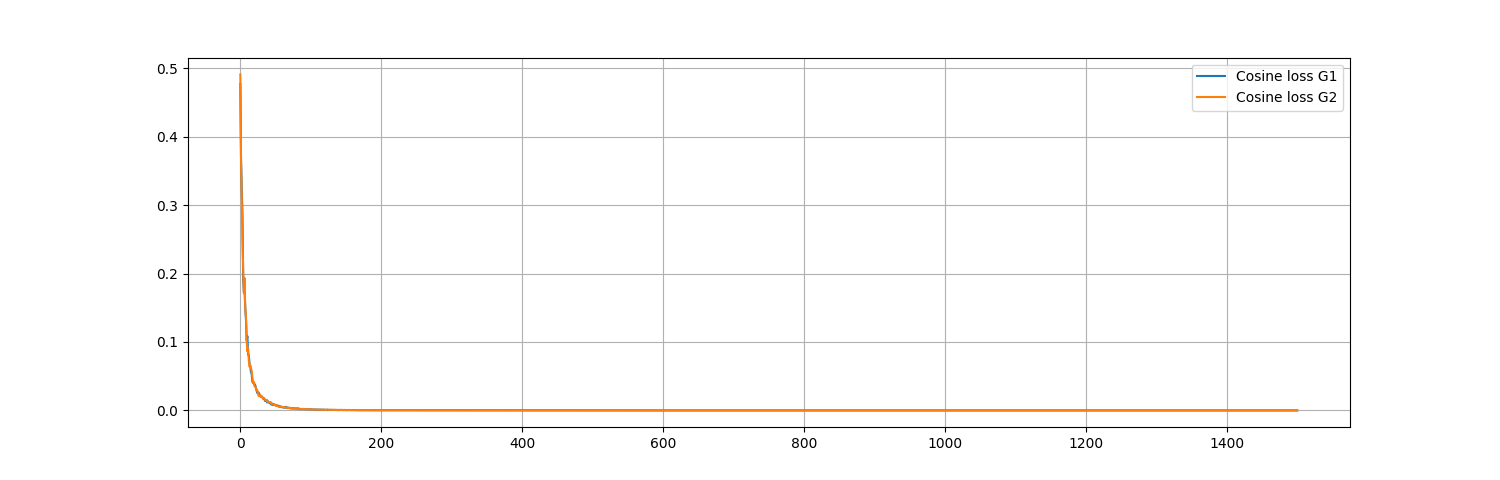
\includegraphics[width=1\textwidth]{figures/c4_unstable/train_losses/cos_cos/cosine_loss.png}}
    \hfill
    \subfloat[]{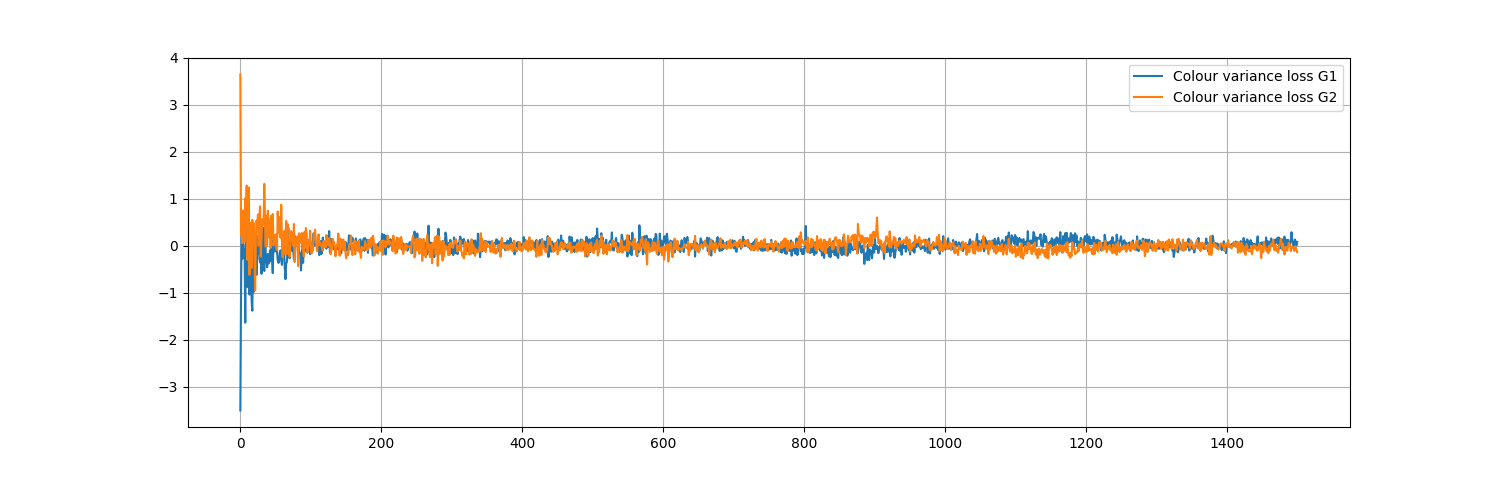
\includegraphics[width=1\textwidth]{figures/c4_unstable/train_losses/cos_cos/col_var_loss.png}}
    \hfill
    \subfloat[]{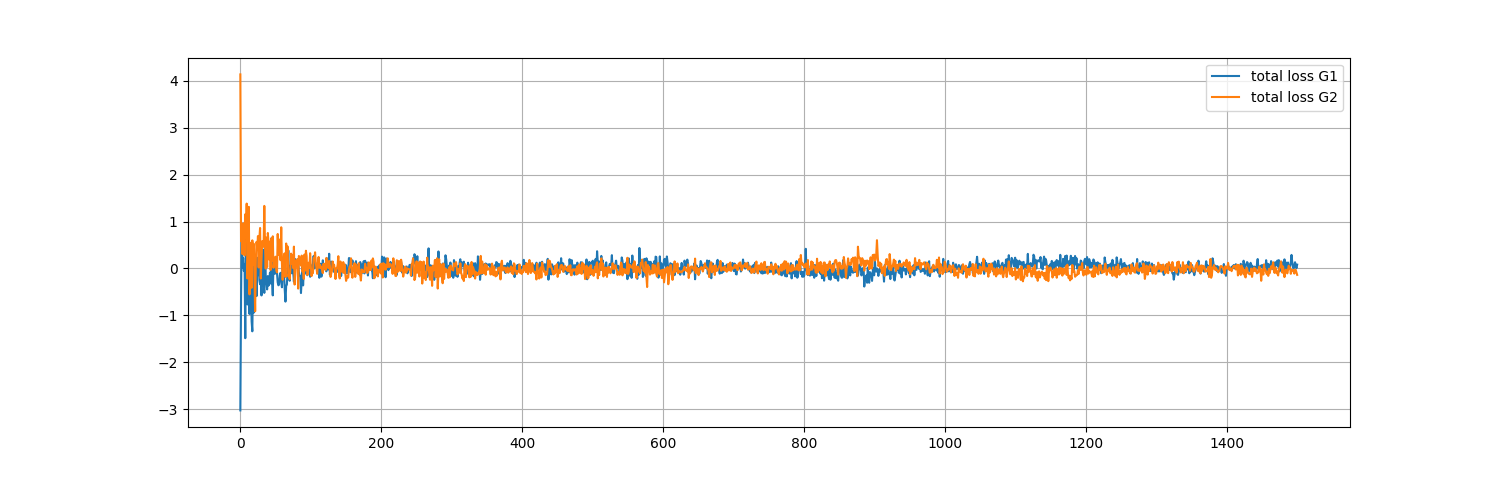
\includegraphics[width=1\textwidth]{figures/c4_unstable/train_losses/cos_cos/total_loss.png}}
    \caption[]{}
    \label{fig:c3:cos-cos-losses}
  \end{figure}

  \section{Euclidean distance}

  \begin{figure}[!htbp]
    \centering
    \subfloat[]{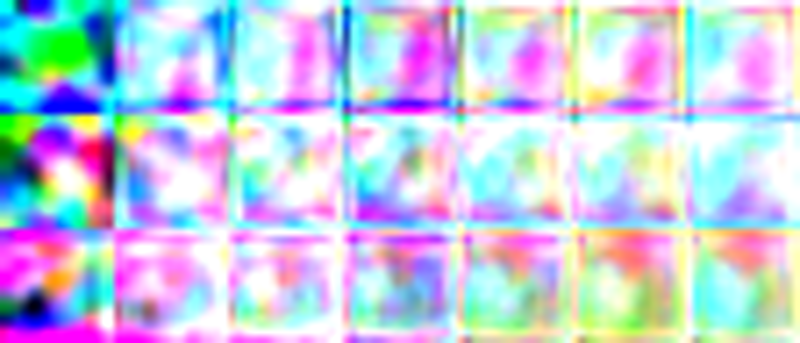
\includegraphics[width=0.45\textwidth]{figures/c4_unstable/train_samples/euclid_euclid/scaled_step_2_g1.png}}
    \hfill
    \subfloat[]{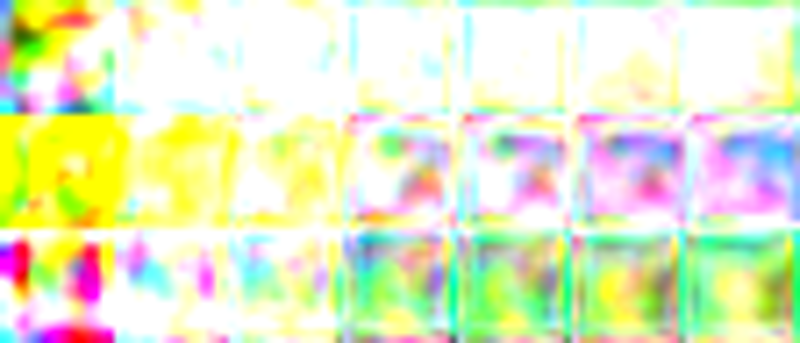
\includegraphics[width=0.45\textwidth]{figures/c4_unstable/train_samples/euclid_euclid/scaled_step_2_g2.png}}
    \hfill
    \subfloat[]{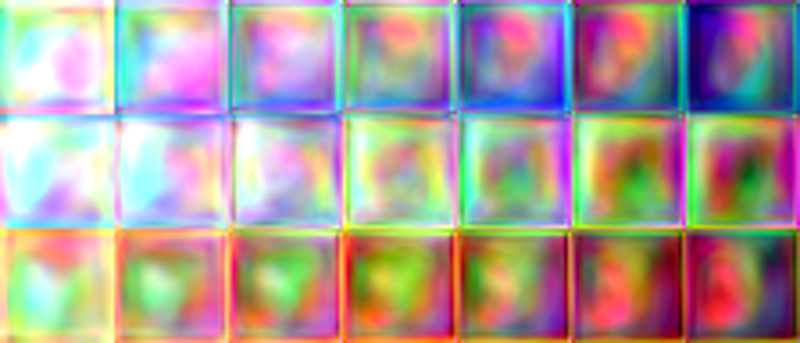
\includegraphics[width=0.45\textwidth]{figures/c4_unstable/train_samples/euclid_euclid/scaled_step_3_g1.png}}
    \hfill
    \subfloat[]{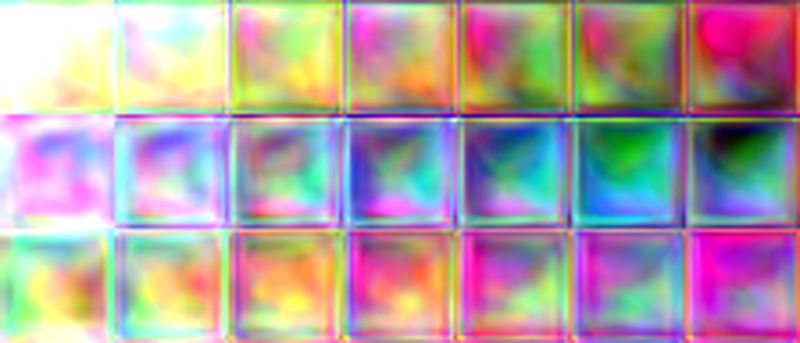
\includegraphics[width=0.45\textwidth]{figures/c4_unstable/train_samples/euclid_euclid/scaled_step_3_g2.png}}
    \hfill
    \subfloat[]{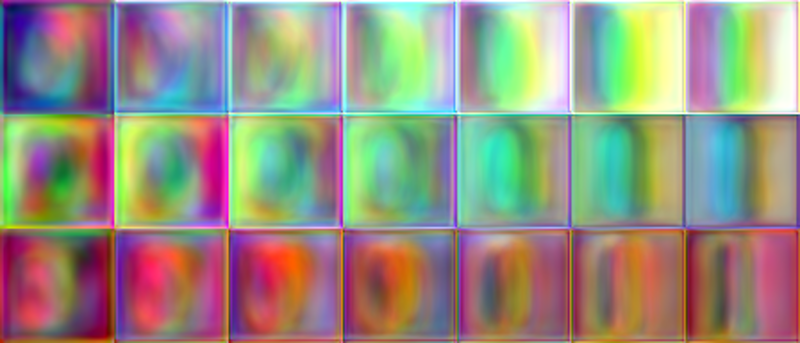
\includegraphics[width=0.45\textwidth]{figures/c4_unstable/train_samples/euclid_euclid/scaled_step_4_g1.png}}
    \hfill
    \subfloat[]{\includegraphics[width=0.45\textwidth]{figures/c4_unstable/train_samples/euclid_euclid/scaled_step_4_g2.png}}
    \hfill
    \subfloat[]{\includegraphics[width=0.45\textwidth]{figures/c4_unstable/train_samples/euclid_euclid/scaled_step_5_g1.png}}
    \hfill
    \subfloat[]{\includegraphics[width=0.45\textwidth]{figures/c4_unstable/train_samples/euclid_euclid/scaled_step_5_g2.png}}
    \hfill
    \subfloat[]{\includegraphics[width=0.45\textwidth]{figures/c4_unstable/train_samples/euclid_euclid/scaled_step_6_g1.png}}
    \hfill
    \subfloat[]{\includegraphics[width=0.45\textwidth]{figures/c4_unstable/train_samples/euclid_euclid/scaled_step_6_g2.png}}
    \hfill
    \caption[]{}
    \label{fig:c3:samples-euclid-euclid}
  \end{figure}

  \begin{figure}[!htbp]
    \centering
    \subfloat[]{\includegraphics[width=1\textwidth]{figures/c4_unstable/train_losses/euclid_euclid/euclid_loss.png}}
    \hfill
    \subfloat[]{\includegraphics[width=1\textwidth]{figures/c4_unstable/train_losses/euclid_euclid/col_var_loss.png}}
    \hfill
    \subfloat[]{\includegraphics[width=1\textwidth]{figures/c4_unstable/train_losses/euclid_euclid/total_loss.png}}
    \caption[]{}
    \label{fig:c3:euclid-euclid-losses}
  \end{figure}

\section{Mixing generator loss functions}

\subsection{Cosine and adversarial }

\begin{figure}[!htbp]
    \centering
    \subfloat[]{\includegraphics[width=0.45\textwidth]{figures/c4_unstable/train_samples/cosine_euclid/scaled_step_2_g1.png}}
    \hfill
    \subfloat[]{\includegraphics[width=0.45\textwidth]{figures/c4_unstable/train_samples/cosine_adv/scaled_step_2_g2.png}}
    \hfill
    \subfloat[]{\includegraphics[width=0.45\textwidth]{figures/c4_unstable/train_samples/cosine_adv/scaled_step_3_g1.png}}
    \hfill
    \subfloat[]{\includegraphics[width=0.45\textwidth]{figures/c4_unstable/train_samples/cosine_adv/scaled_step_3_g2.png}}
    \hfill
    \subfloat[]{\includegraphics[width=0.45\textwidth]{figures/c4_unstable/train_samples/cosine_adv/scaled_step_4_g1.png}}
    \hfill
    \subfloat[]{\includegraphics[width=0.45\textwidth]{figures/c4_unstable/train_samples/cosine_adv/scaled_step_4_g2.png}}
    \hfill
    \subfloat[]{\includegraphics[width=0.45\textwidth]{figures/c4_unstable/train_samples/cosine_adv/scaled_step_5_g1.png}}
    \hfill
    \subfloat[]{\includegraphics[width=0.45\textwidth]{figures/c4_unstable/train_samples/cosine_adv/scaled_step_5_g2.png}}
    \hfill
    \subfloat[]{\includegraphics[width=0.45\textwidth]{figures/c4_unstable/train_samples/cosine_adv/scaled_step_6_g1.png}}
    \hfill
    \subfloat[]{\includegraphics[width=0.45\textwidth]{figures/c4_unstable/train_samples/cosine_adv/scaled_step_6_g2.png}}
    \hfill
    \caption[]{}
    \label{fig:c3:samples-cosine-adv}
  \end{figure}

  \begin{figure}[!htbp]
    \centering
    \subfloat[]{\includegraphics[width=1\textwidth]{figures/c4_unstable/train_losses/cosine_adv/cosine_adv_loss.png}}
    \hfill
    \subfloat[]{\includegraphics[width=1\textwidth]{figures/c4_unstable/train_losses/cosine_adv/col_var_loss.png}}
    \hfill
    \subfloat[]{\includegraphics[width=1\textwidth]{figures/c4_unstable/train_losses/cosine_adv/total_loss.png}}
    \caption[]{}
    \label{fig:c3:cosine-adv-losses}
  \end{figure}

\subsection{Euclid and adversarial}

\begin{figure}[!htbp]
    \centering
    \subfloat[]{\includegraphics[width=0.45\textwidth]{figures/c4_unstable/train_samples/euclid_adv/scaled_step_2_g1.png}}
    \hfill
    \subfloat[]{\includegraphics[width=0.45\textwidth]{figures/c4_unstable/train_samples/euclid_adv/scaled_step_2_g2.png}}
    \hfill
    \subfloat[]{\includegraphics[width=0.45\textwidth]{figures/c4_unstable/train_samples/euclid_adv/scaled_step_3_g1.png}}
    \hfill
    \subfloat[]{\includegraphics[width=0.45\textwidth]{figures/c4_unstable/train_samples/euclid_adv/scaled_step_3_g2.png}}
    \hfill
    \subfloat[]{\includegraphics[width=0.45\textwidth]{figures/c4_unstable/train_samples/euclid_adv/scaled_step_4_g1.png}}
    \hfill
    \subfloat[]{\includegraphics[width=0.45\textwidth]{figures/c4_unstable/train_samples/euclid_adv/scaled_step_4_g2.png}}
    \hfill
    \subfloat[]{\includegraphics[width=0.45\textwidth]{figures/c4_unstable/train_samples/euclid_adv/scaled_step_5_g1.png}}
    \hfill
    \subfloat[]{\includegraphics[width=0.45\textwidth]{figures/c4_unstable/train_samples/euclid_adv/scaled_step_5_g2.png}}
    \hfill
    \subfloat[]{\includegraphics[width=0.45\textwidth]{figures/c4_unstable/train_samples/euclid_adv/scaled_step_6_g1.png}}
    \hfill
    \subfloat[]{\includegraphics[width=0.45\textwidth]{figures/c4_unstable/train_samples/euclid_adv/scaled_step_6_g2.png}}
    \hfill
    \caption[]{}
    \label{fig:c3:samples-euclid-adv}
  \end{figure}

  \begin{figure}[!htbp]
    \centering
    \subfloat[]{\includegraphics[width=1\textwidth]{figures/c4_unstable/train_losses/euclid_adv/euclid_adv_loss.png}}
    \hfill
    \subfloat[]{\includegraphics[width=1\textwidth]{figures/c4_unstable/train_losses/euclid_adv/col_var_loss.png}}
    \hfill
    \subfloat[]{\includegraphics[width=1\textwidth]{figures/c4_unstable/train_losses/euclid_adv/total_loss.png}}
    \caption[]{}
    \label{fig:c3:euclid-adv-losses}
  \end{figure}

\subsection{Cosine and euclidean }

\begin{figure}[!htbp]
    \centering
    \subfloat[]{\includegraphics[width=0.45\textwidth]{figures/c4_unstable/train_samples/cosine_euclid/scaled_step_2_g1.png}}
    \hfill
    \subfloat[]{\includegraphics[width=0.45\textwidth]{figures/c4_unstable/train_samples/cosine_euclid/scaled_step_2_g2.png}}
    \hfill
    \subfloat[]{\includegraphics[width=0.45\textwidth]{figures/c4_unstable/train_samples/cosine_euclid/scaled_step_3_g1.png}}
    \hfill
    \subfloat[]{\includegraphics[width=0.45\textwidth]{figures/c4_unstable/train_samples/cosine_euclid/scaled_step_3_g2.png}}
    \hfill
    \subfloat[]{\includegraphics[width=0.45\textwidth]{figures/c4_unstable/train_samples/cosine_euclid/scaled_step_4_g1.png}}
    \hfill
    \subfloat[]{\includegraphics[width=0.45\textwidth]{figures/c4_unstable/train_samples/cosine_euclid/scaled_step_4_g2.png}}
    \hfill
    \subfloat[]{\includegraphics[width=0.45\textwidth]{figures/c4_unstable/train_samples/cosine_euclid/scaled_step_5_g1.png}}
    \hfill
    \subfloat[]{\includegraphics[width=0.45\textwidth]{figures/c4_unstable/train_samples/cosine_euclid/scaled_step_5_g2.png}}
    \hfill
    \subfloat[]{\includegraphics[width=0.45\textwidth]{figures/c4_unstable/train_samples/cosine_euclid/scaled_step_6_g1.png}}
    \hfill
    \subfloat[]{\includegraphics[width=0.45\textwidth]{figures/c4_unstable/train_samples/cosine_euclid/scaled_step_6_g2.png}}
    \hfill
    \caption[]{}
    \label{fig:c3:samples-cosine-euclid}
  \end{figure}

  \begin{figure}[!htbp]
    \centering
    \subfloat[]{\includegraphics[width=1\textwidth]{figures/c4_unstable/train_losses/cosine_euclid/cosine_euclid_loss.png}}
    \hfill
    \subfloat[]{\includegraphics[width=1\textwidth]{figures/c4_unstable/train_losses/cosine_euclid/col_var_loss.png}}
    \hfill
    \subfloat[]{\includegraphics[width=1\textwidth]{figures/c4_unstable/train_losses/cosine_euclid/total_loss.png}}
    \caption[]{}
    \label{fig:c3:cosine-euclid-losses}
  \end{figure}

In this following approach, I took to the idea of again riffing on the GAN framework, but in this instance, replacing the data component of the framework with another generator. 
The generators are both being optimised to have their outputs has been passed off as the other network, while the discriminator is acting in the standard adversarial fashion as a binary classifier trying to correctly classify the images from each network (See Fig 4). 

\textbf{Figure 4: 2 Generator framework}

Both generators in this framework are still using an adversarial loss, being optimised to trick the discriminator into making the wrong classification, while the discriminator is being optimised to make a correct classification. 
It was clear this arrangement was an immediate improvement from the previous one, in the sense that there is no obvious failure condition where learning will instantly stop, and in this sense it more closely resembles what observes of GANs show as being one of the few learning algorithms in ML that has no defined point it is optimising towards \citep{nagarajan2017gradient}. 
Rather, GANs exist as a dynamical system with no defined end, making it the perfect starting point for these experiments. 
It was clear from the previous experiment that I needed some kind of dynamics between models that would produce some kind of stochastic process, in lieu of data, to generate ‘learning’ dynamics sufficient that the networks significantly diverge from the original state of random initialisation for a styleGAN model. 

\textbf{Figure 5: Random initialised styleGAN}

The first set of training runs produced nothing special. 
There were definitely dynamics between the models leading to interesting changes to the model weights, clearly evident by observing the outputs at each time step (see Fig 6). 
But ultimately, the models converged into a form of mode collapse where the network solely generated one mode of output. 

\textbf{Figure 6: Batch after training (and over time?)}

To deal with this issue, I started thinking of possible ways to overcome the mode collapse state of the model. 
Though the dynamics of training were visually interesting, the goal of training a generative neural networks is to model a distribution, not a single image \footnote{with some notable exceptions, i.e. CPPNs, other ways of modelling individual images with one network}. 
Therefore I need to find a way of pushing this system to have some kind of diversity in the outputs it was creating. In keeping with the ideas of adversarial learning where the networks play off against each other, I decided I could get the generators to compete to produce more colours than the other network in their mini-batch. 
That way, the training dynamics are still from within the arrangements of the networks themselves, and not relying on any external input of what colours are ‘good’.

The additional loss term added to force increased colours to be used was to measure the batch-wide variance of values for each pixel, in each channel of the tensor. 
This term calculates the variance across the sampled batch B for the respective channel c of the tensor for the samples drawn from both generators g1 and g2, which are then subtracted from each other (depending on which loss is being calculated for which generator) to enforce a relative variance that is higher than the other model across the different channels of the sample tensor.

\begin{equation}
    \label{eq:variance-gan}
    Vdiff = Var(B_{g^{1}}^{c}) - Var(B_{g^{2}}^{c})
    \end{equation}

This is calculated for the 4 channels of the tensor present in the sample batch. 
The first channel is the overall batch bt, the following channels are the colour channels of the output images: red r, green g and blue b.

\begin{equation}
    \label{eq:total-gan}
        Vdiff(B_{g^{1}}^{bt} , B_{g^{2}}^{bt}) + Vdiff(B_{g^{1}}^{r} , B_{g^{2}}^{r}) + Vdiff(B_{g^{1}}^{g} , B_{g^{2}}^{g}) + + Vdiff(B_{g^{1}}^{b} , B_{g^{2}}^{b}) 
    \end{equation}

The loss penalty was calculated for each generator with respect to the other. 
Therefore each generator was optimised to have more mini-batch variance than the other. 
Adding this term made a significant impact to the training. 
The networks showed the similar behaviour of having blobs changing over time, but this time maintaining the diversity in the mini-batches (See figure 7). 

\textbf{Figure 7: Training over time}

When sampling the results from the final model, it is clear to see that diversity in the generator output for both models is much greater. 
The spatial structure remains largely consistent throughout, but there is a seemingly endless variation in the colours and combinations of colours generated by the models (see next fig).

\textbf{Figure 8: Latent interp of first model}

The results from this experiment were surprising, to say the least. 
My immediate reaction was to think something along the lines of “wow, that really looks like a Mark Rothko painting”. 
This was not the goal of this work, I had no idea how the images would turn out and I had no real predefined idea in my head of what I wanted. 
Perhaps my aesthetic judgement guided me towards developing a training system that optimises towards this in some way, but I wouldn't particularly call myself a Rothko fan. 

Besides the resemblance to Rothko’s work, what was most striking for me was the seeming use of complementary colours in the images generated by the models \footnote{I recall a conversation I had with Professor Matthew Fuller where I showed him these images and he lamented the fact that a computer could generate something that was so tasteful.} 
There were no mathematical theories used for determining complementary and contracting colours that the model was using, this the simple constraint of pixel-wide variance for each channel across a mini-batch. 
One of the indirect compliments I got from this was a woman at NeurIPS who was convinced that I must have used some kind of data derived from the American colour field painting artistic movement when training the models.

\section{Following Experiments}

After finding a configuration that produced aesthetically interesting results I wanted to explore this framework further. 
In the following experiments, I took to using variations on the original configuration that I set up. 
One element of that was to take variations of distances and similarity measurements, in lieu of simply using the binary classification loss from the original discriminator binary cross entropy loss. 
This included using the cosine similarity/distance (as used in the first experiment detailed in the chapter), as well as the MSE loss (check this?). 
The first and second training runs used the same original setup, while the 3rd-6th training runs used different combinations of these functions for measuring distance and difference. 
The configurations for all training are listed in the table below:

\textbf{Table 1: overview of experiments}

\textit{Following paragraph to fully explain the table.}

The variation in results from these training was quite surprising (See figure 9). 
Even with the first and second training run using the same loss functions, the outcome results are quite distinct for each. 
For 1:3 and 1:4 that use X, the colours are very different, much darker, and the shapes are less band-like and more blob-like. 
1:5 and 1:6 are closer to the original runs, but this time losing their orthogonality. 

\textbf{Figure 9: All of the experimental results}


\section{Discussion}

The results from the experiments presented here show that it is in fact possible to train a generative neural network, without data, such that it produces both surprising and aesthetically interesting outcomes. 
The process described here of iterative development, observing loss functions and iteratively observing the samples generated at each time step, I was primarily looking to arrange a network configuration that had the right kind of dynamics to invoke interesting changes to the weights of the model, and in turn the generated outputs over time. 
As it is a generative system, closely observing what is being generated, and how that changes over training, seemed like the obvious way to monitor progress. 
It didn’t matter what the system was optimising towards, as long as training gradients stayed in the `sweet spot’, neither vanishing nor exploding, and the dynamics of training were in turn leading to interesting developments in the process of training. 

Maintaining gradients to be in this ‘sweet spot’ came with its challenges. 
Normally, stochasticity is present in the data, which is randomly sampled in mini-batches and optimised on using stochastic gradient descent. 
Here SGD and mini-batches were used for training, but there was no data to induce stochasticity into training. 
One of the challenges I set myself in training was to not rely on external information in training or inject any external stochastic process into training either. 
All of the stochasticity had to come the random initialisation of the network models, and from the dynamics between models in training. 
Too high a batch size was detrimental to ensuring there was enough stochasticity in training \footnote{This is not normally the case with training generative models, where the received wisdom is that the higher the batch size, the better}. 
With a very large batch size measurements would get too averaged out, and the dynamics in training would be flattened out. 

Using measurements that were constrained to within a batch, and measuring the difference between models and variation from within a single models batch became an important way of inducing dynamics in training that would lead to interesting results. 
By using slight variations of measuring distance and difference between batches, that also was able to induce some of the stochasticity needed to induce transformative dynamics in the system. 
Again, finding the right batch size was important for this and there was definitely a sweet spot of around 5 where the dynamics were just random enough to induce dynamics that quickly changed the weights of the model. 
\textbf{Expain on the impact of batch size changing over training}.

\section{Conclusion}

The work in this chapter was significant for a number of reasons, the artistic value and its impact in the artwork has already been mentioned. 
From the perspective of the narrative of this thesis though it was important for other reasons. 
This was the first breakthrough in the aim of developing a data-divergent, or more appropriately a data-agnostic way of training generative neural networks, such that they create something completely novel. 
The way this was achieved, leaning on my (relatively) significant experience of coding and training machine learning system, which I had grown to be quite comfortable with, to the degree that I could playfully experiment with the code, without anxiety, and with the ability of quickly building neural networks frameworks where gradient based learning was able to perform successfully.

A number of orthodoxies of machine learning are deliberately challenged in this work. 
The first, that data is needed to ‘learn’ or happen upon culturally relevant representations. That optimisation must be convex, that the goal of optimization must be clearly defined in a formula derived from a theory taken from statistics, physics or some branch of mathematics. 
That regularisation of training comes from the stochastic nature of data, and not from the dynamics of the models themselves. 
That high batch sizes and training for long periods is needed to produce high fidelity results. 
That the loss function needs to go down, and this needs to be observed over long periods of time.

The following chapter builds on this work, though instead of focusing on training models from scratch, I took my next experiments into fine-tuning models that had already been trained.